\chapter{优化程序性能}

编写高效程序需要做到以下几点:第一,我们必须选择一组适当的算法和数据结构。第二,我们必须编写出编译器能够有效优化以转换成高效可执行代码的源代码。第三,针对处理运算量特别大的计算,将一个任务分成多个部分,这些部分可以在多核和多处理器的某种组合上并行地计算。对于第二点,理解优化编译器的能力和局限性是很重要的。

理想的情况是,编译器能够接受我们编写的任何代码,并产生尽可能高效的、具有指定行为的机器级程序。现代编译器采用了复杂的分析和优化形式,然而,即使是最好的编译器也受到 optimization blocker 的阻碍。程序员必须编写容易优化的代码,以帮助编译器。

程序优化的第一步就是消除不必要的工作,让代码尽可能有效地执行所期望的任务。这包括消除不必要的函数调用、内存条件测试和内存引用。这些优化不依赖于目标机器的任何具体属性。为了使程序性能最大化,程序员和编译器都需要一个目标机器的模型,指明如何处理指令,以及各个操作的时序特性。了解了处理器的运作,我们就可以进行程序优化的第二部,利用处理器提供的 instruction-level parallelism 能力,同时执行多条指令。

研究程序的汇编代码表示是理解编译器以及产生的代码会如何运行的最有效手段之一。仔细研究内循环的代码是一个很好的开端,识别出降低性能的属性,例如过多的内存引用和对寄存器使用不当。从汇编代码开始,我们还可以预测什么操作会并行执行,以及它们会如何使用处理器资源。常常会通过确认 critical path 来决定执行一个循环所需要的时间。

\section{优化编译器的能力和局限性}

现代编译器运用复杂精细的算法来确定一个程序中计算的是什么值,以及它们是被如何使用的,然后利用一些机会来简化表达式。

编译器必须很小心地对程序只使用安全的优化,也就是说对于程序可能遇到的所有可能的情况,优化后得到的程序和未优化的版本有一样的行为。例如:

\begin{minted}{cpp}
void twiddle1(long *xp, long *yp) {
  *xp += *yp;
  *xp += *yp;
}

void twiddle2(long *xp, long *yp) {
  *xp += 2 * *yp;
}
\end{minted}

看起来,这两个过程似乎有相同的行为。不过考虑 xp 等于 yp 的情况。此时,函数 twiddle1 会执行下面的计算:

\begin{minted}[autogobble=false, firstnumber=2]{cpp}
  *xp += *xp;  // Double value at xp
  *xp += *xp;  // Double value at xp
\end{minted}
结果是 xp 的值增加 4 倍。另一方面,函数 twiddle2 会执行下面的计算:

\begin{minted}[autogobble=false, firstnumber=7]{cpp}
  *xp += 2 * *xp;  // Triple value at xp
\end{minted}
结果是 xp 的值增加 3 倍。编译器不知道 twiddle 会如何被调用,因此它必须假设参数 xp 和 yp 可能会相等。因此,它不能产生 twiddle2 风格的代码作为 twiddle1 的优化版本。

这种两个指针可能指向同一个内存位置的情况称为 memory aliasing。在只执行安全的优化中,编译器必须假设不同的指针可能会指向内存中同一个位置。

这造成了一个主要的 optimization blocker,这也是可能严重限制编译器产生优化代码机会的程序的一个方面。如果编译器不能确定两个指针是否指向同一个位置,就必须假设什么情况都有可能,这就限制了可能的优化策略。

\section{表示程序性能}

我们引入度量标准 Cycles Per Element,CPE,作为一种表示程序性能并指导我们改进代码的方法。CPE 这种度量标准帮助我们在更细节的级别上理解迭代程序的循环性能。

\section{程序示例}

为了说明一个抽象的程序是如何被系统地转换成更有效的代码的,我们将使用一个基于下图所示向量数据结构的运行示例。

\begin{tikzfig}
    \coordinate (A) at (0, 0);
    \coordinate (B) at (2, 0);
    \coordinate (C) at (0, -1);
    \coordinate (D) at (B |- C);
    \coordinate (ac1) at ($(A)!1/2!(C)$);
    \coordinate (bd1) at ($(B)!1/2!(D)$);
    \fill[fill=White!80!ProcessBlue] (A) rectangle (D);
    \path (A) rectangle node{len} (bd1);
    \draw (ac1) -- (bd1);
    \draw (A) -- node[left]{len} (ac1) -- node[left]{data} (C) -- (D) -- (B) -- (A);
    \coordinate (E) at ($(bd1) + (2, 0)$);
    \coordinate (F) at ($(E) + (7, 0)$);
    \coordinate (G) at ($(D) + (2, 0)$);
    \coordinate (H) at ($(G) + (7, 0)$);
    \foreach \i in {0, 1, 2, ..., 7} {
        \coordinate (ef\i) at ($(E)!\i/7!(F)$);
        \coordinate (gh\i) at ($(G)!\i/7!(H)$);
    }
    \fill[fill=White!60!gray] (E) rectangle (gh3);
    \fill[fill=White!60!gray] (ef6) rectangle (H);
    \draw (E) -- node[above]{0} (ef1)
              -- node[above]{1} (ef2)
              -- node[above]{2} (ef3)
              -- (ef6)
              -- node[above]{len-1} (F)
              -- (H) -- (G) -- (E);
    \draw (ef1) -- (gh1);
    \draw (ef2) -- (gh2);
    \draw (ef3) -- (gh3);
    \draw (ef6) -- (gh6);
    \path (ef3) rectangle node{. . .} (gh6);
    \coordinate (K) at ($(bd1)!1/2!(D) - (0.2, 0)$);
    \fill (K) circle[radius=1pt];
    \draw[-latex] (K) -- ($(E)!1/2!(G)$);
\end{tikzfig}

向量由两个内存块表示:头部和数据数组。头部是一个声明如下的结构:

\begin{minted}{cpp}
// vec.h
// Create abstract data type for vector
typedef struct {
  long len;
  data_t *data;
} vec_rec, *vec_ptr;
\end{minted}

这个声明用 \verb|data_t| 来表示基本元素的数据类型。在测试中,我们度量代码对于整数和浮点数数据的性能。

下面给出了一些生成向量、访问向量元素以及确定向量长度的基本过程:

\begin{minted}{cpp}
// Create vector of specified length
vec_ptr new_vec(long len) {
  // Allocate header structure
  vec_ptr result = (vec_ptr)malloc(sizeof(vec_rec));
  data_t *data = NULL;
  if (!result) return NULL; // Couldn't allocate storage
  result->len = len;
  // Allocate array
  if (len > 0) {
    data = (data_t*)calloc(len, sizeof(data_t));
    if (!data) {
      free((void*)result);
      return NULL; // Couldn't allocate storage
    }
  }
  // Data will either be NULL or allocated storage
  result->data = data;
  return result;
}

// Retrieve vector element and store at dest
// Return 0 (out of bounds) or 1 (successful)
int get_vec_element(vec_ptr v, long index, data_t *dest) {
  if (index < 0 || index >= v->len) return 0;
  *dest = v->data[index];
  return 1;
}

// Return length of vector
long vec_length(vec_ptr v) {
  return v->len;
}
\end{minted}

作为一个优化示例,考虑如下代码:

\begin{minted}{cpp}
// Implementation with maximum use of data abstraction
void combine1(vec_ptr v, data_t *dest) {
  long i;
  *dest = IDENT;
  for (i = 0; i < vec_length(v); i++) {
    data_t val;
    get_vec_element(v, i, &val);
    *dest = *dest OP val;
  }
}
\end{minted}

它使用某种运算,将一个数组中所有的元素合并成一个值。通过使用编译时常数 IDENT 和 OP 的不同定义,这段代码可以重编译成对数据执行不同的运算。特别的,使用声明:
\begin{minted}{cpp}
#define IDENT 0
#define OP +
\end{minted}
它对数组的元素求和。使用声明:
\begin{minted}{cpp}
#define IDENT 1
#define OP *
\end{minted}
它计算的是数组元素的乘积。

作为一个起点,下表给出的是 combine1 的 CPE 度量值,它运行在参考机上,尝试了操作(加法或乘法)和数据类型(整数或浮点数)的不同组合。

\begin{table}[!ht]
    \centering
    \begin{tabular}{llccccc}
        \toprule
        & & \multicolumn{2}{c}{Integer} & & \multicolumn{2}{c}{Floating point} \\
        \cmidrule{3-4} \cmidrule{6-7}
        Function & Method & + & * & & + & * \\
        \midrule
        \texttt{combine1} & Abstract unoptimized & 22.68 & 20.02 & & 19.98 & 20.18 \\
        \texttt{combine1} & Abstract -O1 & 10.12 & 10.12 & & 10.17 & 11.14 \\
        \bottomrule
    \end{tabular}
\end{table}

\section{消除循环的低效率}

可以观察到,过程 combine1 调用函数 \verb|vec_length| 作为 for 循环的测试条件,每次循环迭代时都必须对测试条件求值。另一方面,向量的长度并不会随着循环的进行而改变。因此,只需计算一次向量的长度。

\begin{minted}{cpp}
// Move call to vec_length out of loop
void combine2(vec_ptr v, data_t *dest) {
  long i;
  long length = vec_length(v);
  *dest = IDENT;
  for (i = 0; i < length; i++) {
    data_t val;
    get_vec_element(v, i, &val);
    *dest = *dest OP val;
  }
}
\end{minted}

\begin{table}[!ht]
    \centering
    \begin{tabular}{llccccc}
        \toprule
        & & \multicolumn{2}{c}{Integer} & & \multicolumn{2}{c}{Floating point} \\
        \cmidrule{3-4} \cmidrule{6-7}
        Function & Method & + & * & & + & * \\
        \midrule
        \texttt{combine1} & Abstract -O1 & 10.12 & 10.12 & & 10.17 & 11.14 \\
        \texttt{combine2} & Move \texttt{vec\_length} & 7.02 & 9.03 & & 9.02 & 11.03 \\
        \bottomrule
    \end{tabular}
\end{table}

这个优化是一类常见的优化,称为 code motion(代码移动)。这类优化包括识别要执行多次但是计算结果不会改变的计算。因而可以将计算移动到代码前面不会被多次求值的部分。

\section{减少过程调用}

过程调用会带来开销,而且妨碍大多数形式的程序优化。从 combine2 的代码中我们可以看出,每次循环迭代都会调用 \verb|get_vec_element| 来获取下一个向量元素。对每个向量引用,这个函数要把向量索引 i 与循环边界做比较,很明显会降低效率。在处理任意的数组访问时,边界检查很有用,但是对 combine2 代码的简单分析表明,所有的引用都是合法的。

作为替代,假设为我们的抽象数据类型增加一个函数 \verb|get_vec_start|。这个函数返回数组的起始地址,然后就能写出下面的 combine3 所示的过程,其内循环里没有函数调用。它没有用函数调用来获取每个向量元素,而是直接访问数组。

\begin{minted}{cpp}
data_t *get_vec_start(vec_ptr v) {
  return v->data;
}
\end{minted}

\begin{minted}{cpp}
// Direct access to vector data
void combine3(vec_ptr v, data_t *dest) {
  long i;
  long length = vec_length(v);
  data_t *data = get_vec_start(v);
  *dest = IDENT;
  for (i = 0; i < length; i++) {
    *dest = *dest OP data[i];
  }
}
\end{minted}

\begin{table}[!ht]
    \centering
    \begin{tabular}{llccccc}
        \toprule
        & & \multicolumn{2}{c}{Integer} & & \multicolumn{2}{c}{Floating point} \\
        \cmidrule{3-4} \cmidrule{6-7}
        Function & Method & + & * & & + & * \\
        \midrule
        \texttt{combine2} & Move \texttt{vec\_length} & 7.02 & 9.03 & & 9.02 & 11.03 \\
        \texttt{combine3} & Direct data access & 7.17 & 9.02 & & 9.02 & 11.03 \\
        \bottomrule
    \end{tabular}
\end{table}

令人吃惊的是,性能没有明显的提升。事实上,整数求和的性能还略有下降。显然,内循环中的其他操作形成了瓶颈,限制性能超过调用 \verb|get_vec_element|。我们还会再回到这个函数(5.11.2 节),看看为什么 combine2 中反复的边界检查不会让性能更差。

\section{消除不必要的内存引用}

combine3 的代码将合并运算计算的值累积在指针 \verb|dest| 指定的位置。通过检查编译出来的为内循环产生的汇编代码,可以看出这一行为。在此我们给出数据类型为 double,合并运算为乘法的 x86-64 代码:

\begin{minted}{gas}
# Inner loop of combine3. data_t = double, OP = *. Compiled by clang -O1.
# dest in %rbx, data in %rax, i in %rcx, length in %r14
.LBB6_2:                            # loop:
    movsd   (%rbx), %xmm0           #   Read product from dest
    mulsd   (%rax,%rcx,8), %xmm0    #   Multiply product by data[i]
    movsd   %xmm0, (%rbx)           #   Store product at dest
    addq    $1, %rcx                #   Increment i
    cmpq    %rcx, %r14              #   Comapre to length
    jne .LBB6_2                     #   if !=, goto loop
\end{minted}

可以看到每次迭代时,累积变量的数值都要从内存读出再写入到内存。这样的读写很浪费,因为每次迭代开始时从 \verb|dest| 读出的值就是上次迭代最后写入的值。我们能够消除这种不必要的内存读写,按照如下 combine4 所示的方式重写代码。引入一个临时变量 \verb|acc|,它在循环中用来累积计算出来的值。只有在循环完成之后才将结果存放到 \verb|dest| 中。

\begin{minted}{cpp}
// Accumulate result in local variable
void combine4(vec_ptr v, data_t *dest) {
  long i;
  long length = vec_length(v);
  data_t *data = get_vec_start(v);
  data_t acc = IDENT;
  for (i = 0; i < length; i++) {
    acc = acc OP data[i];
  }
  *dest = acc;
}
\end{minted}

\begin{minted}{gas}
# Inner loop of combine4. data_t = double, OP = *. Compiled by clang -O1.
# acc in %xmm0, data in %rax, i in %rcx, length in %rbx
.LBB7_2:                            # loop:
    mulsd   (%rax,%rcx,8), %xmm0    #   Multiply acc by data[i]
    addq    $1, %rcx                #   Increment i
    cmpq    %rcx, %rbx              #   Compare to length
    jne .LBB7_2                     #   if !=, goto loop
\end{minted}

与 combine3 中的循环相比,我们将每次迭代的内存操作从两次读和一次写减少到只需要一次读。

\begin{table}[!ht]
    \centering
    \begin{tabular}{llccccc}
        \toprule
        & & \multicolumn{2}{c}{Integer} & & \multicolumn{2}{c}{Floating point} \\
        \cmidrule{3-4} \cmidrule{6-7}
        Function & Method & + & * & & + & * \\
        \midrule
        \texttt{combine3} & Direct data access & 7.17 & 9.02 & & 9.02 & 11.03 \\
        \texttt{combine4} & Accumulate in temporary & 1.27 & 3.01 & & 3.01 & 5.01 \\
        \bottomrule
    \end{tabular}
\end{table}

需要注意的是,由于内存别名问题,combine3 和 combine4 在某些情况可能会有不同的行为,所以编译器会采用保守的策略,不会自动将 combine3 优化为 combine4,,尽管 combine4 的行为更加符合函数描述的意图。

当用带命令行选项 -O2 编译 combine3 时,得到的代码 CPE 性能远好于使用 -O1 时:

\begin{table}[!ht]
    \centering
    \begin{tabular}{llccccc}
        \toprule
        & & \multicolumn{2}{c}{Integer} & & \multicolumn{2}{c}{Floating point} \\
        \cmidrule{3-4} \cmidrule{6-7}
        Function & Method & + & * & & + & * \\
        \midrule
        \texttt{combine3} & Compiled -O1 & 7.17 & 9.02 & & 9.02 & 11.03 \\
        \texttt{combine4} & Compiled -O2 & 1.60 & 3.01 & & 3.01 & 5.01 \\
        \texttt{combine4} & Accumulate in temporary & 1.27 & 3.01 & & 3.01 & 5.01 \\
        \bottomrule
    \end{tabular}
\end{table}

在检查编译器产生的汇编代码时,我们发现内循环的一个有趣的变化:

\begin{minted}{gas}
# Inner loop of combine3. data_t = double, OP = *. Compiled by clang -O2.
# dest in %rsi, data in %rcx, i in %rdx, length in %rax
.LBB6_7:                            # loop:
    mulsd   (%rcx,%rdx,8), %xmm0    #   Multiply product by data[i]
    movsd   %xmm0, (%rsi)           #   Store product at dest
    addq    $1, %rdx                #   Increment i
    cmpq    %rdx, %rax              #   Compare to length
    jne .LBB6_7                     #   if !=, goto loop
\end{minted}

把上面的代码与用 -O1 产生的代码进行比较:

\begin{minted}{gas}
# Inner loop of combine3. data_t = double, OP = *. Compiled by clang -O1.
# dest in %rbx, data in %rax, i in %rcx, length in %r14
.LBB6_2:                            # loop:
    movsd   (%rbx), %xmm0           #   Read product from dest
    mulsd   (%rax,%rcx,8), %xmm0    #   Multiply product by data[i]
    movsd   %xmm0, (%rbx)           #   Store product at dest
    addq    $1, %rcx                #   Increment i
    cmpq    %rcx, %r14              #   Comapre to length
    jne .LBB6_2                     #   if !=, goto loop
\end{minted}

我们看到,-O2 中减少了一条 \verb|movsd| 指令,直接从 \verb|dest| 指定的位置读数据。

\section{理解现代处理器}

到目前为止,我们运用的优化都不依赖于目标机器的任何特性。这些优化只是简单地降低了过程调用的开销,以及消除了一些重大的 optimization blocker,这些因素会给优化编译器造成困难。随着试图进一步提高性能,必须考虑利用处理器微体系结构的优化,也就是处理器用来执行指令的底层系统设计。要想充分提高性能,需要仔细分析程序,同时代码的生成也要针对目标处理器进行调整。

为了理解改进性能的方法,我们需要理解现代处理器的微体系结构。在代码级上,看上去似乎是一次执行一条指令,每条指令都包括从寄存器或内存取值,执行一个操作,并把结果存回到一个寄存器或内存位置。在实际的处理器中,是同时对多条指令求值的,这个现象称为指令级并行。

我们会发现两种下界描述了程序的最大性能。当一系列操作必须按照严格顺序执行时,就会遇到 latency bound(延迟界限),因为在下一条指令开始之前,这条指令必须结束。当代码中的数据相关限制了处理器利用指令级并行的能力时,延迟界限能够限制程序性能。throughput bound(吞吐量界限)刻画了处理器功能单元的原始计算能力,这个界限是程序性能的终极限制。

\subsection{整体操作}

下图是现代微处理器的一个非常简单化的示意图。这些处理器在工业界称为 superscalar,意思是它可以在每个始终周期执行多个操作,而且是 out-of-order 的,意思就是指令执行的数序不一定要与它们在机器级程序中的顺序一致。整个设计有两个主要部分,Instruction Control Unit,ICU 和 Execution,EU。前者负责从内存中读出指令序列,并根据这些指令序列生成一组针对程序数据的基本操作;而后者执行这些操作。

\begin{figure}[!ht]
    \centering
    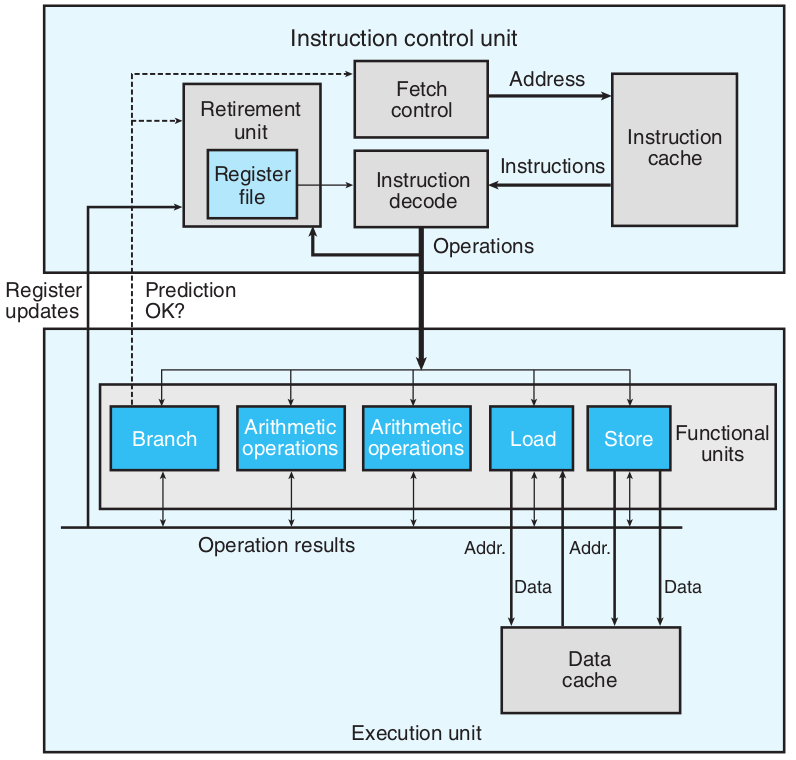
\includegraphics[scale=0.5]{img/5-1}
\end{figure}

ICU 从 instruction cache 中读取指令,icache 是一个特殊的高速存储器,它包含最近访问的指令。通常,ICU 会在当前正在执行的指令很早之前取指,这样它才有足够的之间对指令译码,并把操作发送到 EU。不过,一个问题是当程序遇到分支时,程序有两个可能的前进方向。现代处理器采用了一种称为 branch prediction 的技术,处理器会猜测是否会选择分支,同时还预测分支的目的地址。使用 speculative execution 的技术,处理器会开始取出位于它预测的分支会跳到的地方的指令,并对指令译码,甚至在它确定分支预测是否正确之前就开始执行这些操作。如果过后确定分支预测错误,会将状态重新设置到分支点的状态,并开始取出和执行另一个方向上的指令。

指令译码逻辑接收实际的程序指令,并将它们转换成一组基本操作(有时称为微操作)。

EU 接收来自取指单元的操作。通常,每个时钟周期会接收多个操作。这些操作会被分派到一组功能单元中,它们会执行实际的操作。这些功能单元专门用来处理不同类型的操作。

读写内存是由加载和存储单元实现的,通过 data cache 来访问内存,通过加法器来完成地址计算。

使用投机执行技术对操作求值,但是最终结果不会存放在程序寄存器或数据内存中,直到处理器能够确定应该实际执行这些指令。

在 ICU 中,retirement unit 记录正在进行的处理,并确保它遵守机器级程序的顺序语义。一旦一条指令的操作完成了,而且所有引起这条指令的分支点也都被确认为预测正确,那么这条指令就可以 retired 了,所有对程序寄存器的更新都可以被实际执行了。另一方面,如果引起该指令的某个分支预测点预测错误,这条指令会被 flushed,丢弃所有计算出来的结果。

控制操作数在执行单元间传送的最常见的机制称为 register renaming。

\subsection{功能单元的性能}

下表提供了参考机的一些算术运算的性能。每个运算都是由以下这些数值来刻画的:一个是 latency,它表示完成运算所需要的总时间;另一个是 issue time,它表示两个连续的同类型的运算之间所需要的最小时钟周期数;还有一个是 capacity,它表示能够执行该运算的功能单元的数量。

\begin{table}[!ht]
    \centering
    \begin{tabular}{lccccccc}
        \toprule
        & \multicolumn{3}{c}{Integer} & & \multicolumn{3}{c}{Floating point} \\
        \cmidrule{2-4} \cmidrule{6-8}
        Operation & Latency & Issue & Capacity & & Latency & Issue & Capacity \\
        \midrule
        Addition & 1 & 1 & 4 & & 3 & 1 & 1 \\
        Multiplication & 3 & 1 & 1 & & 5 & 1 & 2 \\
        Division & 3-30 & 3-30 & 1 & & 3-15 & 3-15 & 1 \\
        \bottomrule
    \end{tabular}
\end{table}

发射时间为 1 的功能单元被称为 fully pipelined:每个时钟周期可以开始一个新的运算;出现容量大于 1 的运算是由于有多个功能单元。

表达发射时间的一种更常见的方法是指明这个功能单元的最大吞吐量,定义为发射时间的倒数。一个完全流水化的功能单元有最大的吞吐量,每个时钟周期一个运算,而发射时间较大的功能单元的最大吞吐量较小。具有多个功能单元可以进一步提高吞吐量。对于一个容量为 C,发射时间为 I 的操作来说,处理器可能获得的吞吐量为每时钟周期 C/I 个操作。

这些算术运算的延迟、发射时间和容量会影响我们的 combine 函数的性能。我们用 CPE 值的两个基本界限来描述这种影响:

\begin{table}[!ht]
    \centering
    \begin{tabular}{lccccc}
        \toprule
        & \multicolumn{2}{c}{Integer} & & \multicolumn{2}{c}{Floating point} \\
        \cmidrule{2-3} \cmidrule{5-6}
        Bound & + & * & & + & * \\
        \midrule
        Latency & 1.00 & 3.00 & & 3.00 & 5.00 \\
        Throughput & 0.50 & 1.00 & & 1.00 & 0.50 \\
        \bottomrule
    \end{tabular}
\end{table}

Latency bound 给出了任何必须按照严格顺序完成 combine 运算的函数所需要的最小的 CPE 值。根据功能单元产生结果的最大速率,throughput bound 给出了 CPE 的最小界限。例如,因为只有一个整数乘法器,它的发射时间为 1 个时钟周期,处理器不可能支持每个时钟周期大于 1 条乘法的速度。另一方面,4 个功能单元都可以执行整数加法,处理器就有可能持续每个周期执行 4 个操作的速率,不幸的是,因为需要从内存读数据,这造成了另一个吞吐量界限。2 个加载单元限制了处理器每个时钟周期最多只能读取 2 个数据值,从而使得吞吐量界限为 0.5。

\subsection{处理器操作的抽象模型}

作为分析在现代处理器上执行的机器级程序性能的一个工作,我们会使用程序的 data-flow 表示,这是一种图形化的表示方法,展现了不同操作之间的数据相关是如何限制它们的执行顺序的。这些限制形成了图中的 critical path,这是执行一组机器指令所需时钟周期数的一个下界。

到目前为止,combine4 是最快的代码:

\begin{table}[!ht]
    \centering
    \begin{tabular}{llccccc}
        \toprule
        & & \multicolumn{2}{c}{Integer} & & \multicolumn{2}{c}{Floating point} \\
        \cmidrule{3-4} \cmidrule{6-7}
        Function & Method & + & * & & + & * \\
        \midrule
        \texttt{combine4} & Accumulate in temporary & 1.27 & 3.01 & & 3.01 & 5.01 \\
        Latency bound & & 1.00 & 3.00 & & 3.00 & 5.00 \\
        Throughput bound & & 0.50 & 1.00 & & 1.00 & 0.50 \\
        \bottomrule
    \end{tabular}
\end{table}

\subsubsection{从机器级代码到数据流图}

以 combine4 为例来描述数据流表示法。

\begin{minted}{gas}
# Inner loop of combine4. data_t = double, OP = *. Compiled by gcc -O1.
# acc in %xmm0, data+i in %rdx, data+length in %rax
.L25:                           # loop:
    mulsd   (%rdx), %xmm0       #   Multiply acc by data[i]
    addq    $8, %rdx            #   Increment data+i
    cmpq    %rax, %rdx          #   Compare to data+length
    jne     .L25                #   If !=, goto loop
\end{minted}

\begin{figure}[!ht]
    \centering
    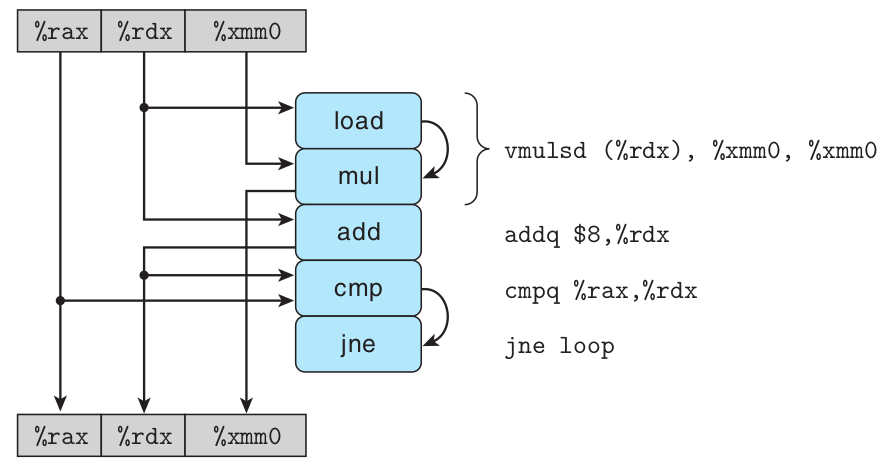
\includegraphics[scale=0.5]{img/5-2}
\end{figure}

对于形成循环的代码片段,我们可以将访问到的寄存器分为 4 类:
\begin{itemize}
    \item Read-only. 这些寄存器只用作源值,可以作为数据,也可以用来计算内存地址,但是在循环中它们是不会被修改的,循环 combine4 的只读寄存器是 \verb|%rax|。
    \item Write-only. 这些寄存器作为数据传送操作的目的。在本循环中没有这样的寄存器。
    \item Local. 这些寄存器在循环内部被修改和使用,迭代与迭代之间不相关。在这个循环中,条件码寄存器就是例子:\verb|cmp| 操作会修改它们,然后 \verb|jne| 操作会使用它们,不过这种相关是在单次迭代之内的。
    \item Loop. 对于循环来说,这些寄存器既作为源值,又作为目的,一次迭代中产生的值会在另一次迭代中用到。可以看到,\verb|%rdx| 和 \verb|%xmm0| 是 combine4 的循环寄存器,对应于程序值 \verb|data+i| 和 \verb|acc|。
\end{itemize}

循环寄存器之间的操作链决定了限制性能的数据相关。

下图是上图的图形化表示的进一步改进,目标是只给除影响程序执行时间的操作和数据相关。图 a 中,重新排列了操作符,更清晰地表明了从顶部源寄存器(只读寄存器和循环寄存器)到底部目的寄存器(只写寄存器和循环寄存器)的数据流。

\begin{figure}[!ht]
    \centering
    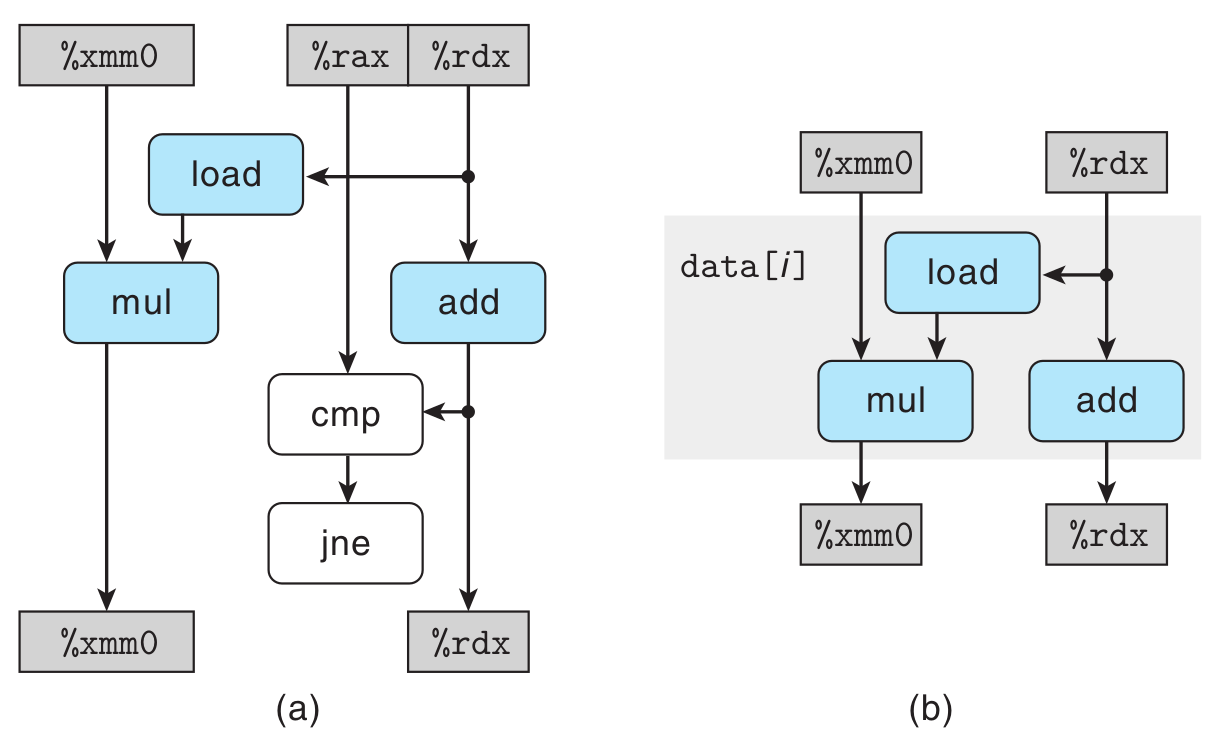
\includegraphics[scale=0.4]{img/5-3}
\end{figure}

图 b 中,消除了左边标识为白色的操作符,而且只保留了循环寄存器。剩下的是一个抽象的模板,表明的是由于循环的一次迭代在循环寄存器中形成的数据相关。在这个图中可以看到,从一次迭代到下一次迭代有 2 个数据相关。在一边,我们看到存储在寄存器 \verb|%xmm0| 中的程序值 \verb|acc| 的连续的值之间有相关。通过将 \verb|acc| 的旧值乘以一个数据元素,循环计算出 \verb|acc| 的新值,这个数据元素是由 \verb|load| 操作产生的。在另一边,我们看到循环索引 \verb|i| 的旧值用来计算 \verb|load| 操作的地址,然后 \verb|add| 操作也会增加它的值,计算出新值。

下图给出了函数 combine4 内循环的 n 次迭代的数据流表示。可以看出,简单地重复上图 b 的模板 n 次,就能得到下图。可以看到,程序有两条数据相关链,分别对应于操作 \verb|mul| 和 \verb|add| 对程序值 \verb|acc| 和 \verb|data+i| 的修改。假设浮点乘法延迟为 5 个周期,而整数加法延迟为 1 个周期,可以看到左边的链会成为关键路径,需要 5n 个周期执行。右边的链只需要 n 个周期执行,因此,它不会制约程序的性能。

\begin{figure}[!ht]
    \centering
    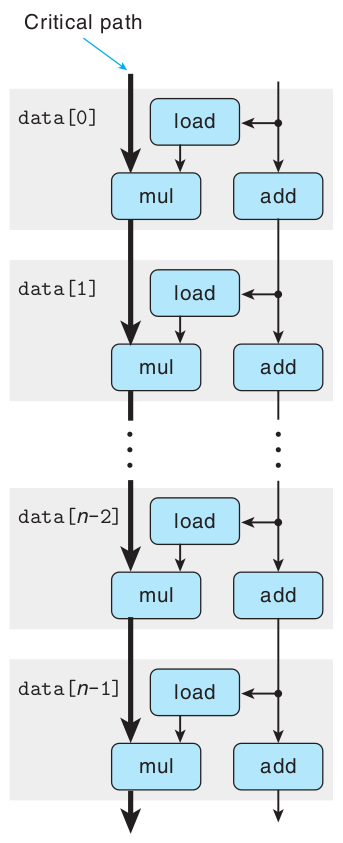
\includegraphics[scale=0.5]{img/5-4}
\end{figure}

\subsubsection{其他性能因素}

另一方面,对于整数加法的情况,我们对 combine4 的测试表明 CPE 为 1.27,而根据上图中左边和右边形成的相关链预测的 CPE 为 1.00,测试值比预测值要慢。这说明了一个原则,那就是数据流表示中的关键路径提供的只是程序需要的周期数的下界。还有其他一些因素会限制性能,包括可用的功能单元的数量和任何一步中功能单元之间能够传递数据值的数量。对于 combine 运算为整数加法的情况,数据操作足够快,使得其他操作供应数据的速度不够快。要准确地确定为什么程序中每个元素需要 1.27 个周期,需要比公开可以获得的更详细的硬件设计知识。

总结一下 combine4 的性能分析:我们对程序操作的抽象数据流表示说明,combine4 的关键路径长 $L \cdot n$ 是由对程序值 \verb|acc| 的连续更新造成的,这条路径将 CPE 限制为最多 L。除了整数加法外,对于所有的其他情况,测量出来的 CPE 确实等于 L,对于整数加法,测量出来的 CPE 为 1.27 而不是根据关键路径的长度所期望的 1.00。

看上去,延迟界限是基本的限制,决定了 combine 运算能执行多快。接下来的任务是重新调整操作的结构,增强指令级并行性。

\section{循环展开}

循环展开是一种程序变换,通过增加每次迭代计算的元素的数量,减少循环的迭代次数。循环展开能够从两个方面改进程序的性能。首先,它减少了不直接有助于程序结果的操作的数量,例如循环索引计算和条件分支。第二,它提供了一些方法,可以进一步变化代码,减少了整个计算中关键路径上的操作数量。

下图是 combine 代码的使用 $2 \times 1$ 循环展开的版本。第一个循环每次处理数组的两个元素,也就是每次迭代,循环索引 $i$ 加 2,在一次迭代中,对数组元素 $i$ 和 $i+1$ 使用 combine 运算。

\begin{minted}{cpp}
// 2 x 1 loop unrolling
void combine5(vec_ptr v, data_t *dest) {
  long i;
  long length = vec_length(v);
  long limit = length - 1;
  data_t *data = get_vec_start(v);
  data_t acc = IDENT;

  // Combine 2 elements at a time
  for (i = 0; i < limit; i += 2) {
    acc = (acc OP data[i]) OP data[i+1];
  }

  // Finish any remaining elements
  for (; i < length; ++i) {
    acc = acc OP data[i];
  }
  *dest = acc;
}
\end{minted}

把这个思想归纳为对一个循环按任意因子 $k$ 进行展开,由此产生 $k \times 1$ 循环展开。

当测量展开次数 $k = 2$ 和 $k = 3$ 的展开代码的性能时,得到下面的结果:

\begin{table}[!ht]
    \centering
    \begin{tabular}{llccccc}
        \toprule
        & & \multicolumn{2}{c}{Integer} & & \multicolumn{2}{c}{Floating point} \\
        \cmidrule{3-4} \cmidrule{6-7}
        Function & Method & + & * & & + & * \\
        \midrule
        \texttt{combine4} & No unrolling & 1.27 & 3.01 & & 3.01 & 5.01 \\
        \texttt{combine5} & $2 \times 1$ unrolling & 1.01 & 3.01 & & 3.01 & 5.01 \\
                          & $3 \times 1$ unrolling & 1.01 & 3.01 & & 3.01 & 5.01 \\
        \\
        Latency bound & & 1.00 & 3.00 & & 3.00 & 5.00 \\
        Throughput bound & & 0.50 & 1.00 & & 1.00 & 0.50 \\
        \bottomrule
    \end{tabular}
\end{table}

可以看到对于整数加法,CPE 有所改进,会有这样的结果是得益于减少了循环开销操作。相对于计算向量和所需要的加法数量,降低开销操作的数量,此时,整数加法的一个周期的延迟成为了限制性能的因素。另一方面,其他情况都已经达到了其延迟界限,并没有性能提高。

\begin{figure}[!ht]
    \centering
    \begin{minipage}{0.65\textwidth}
        \centering
        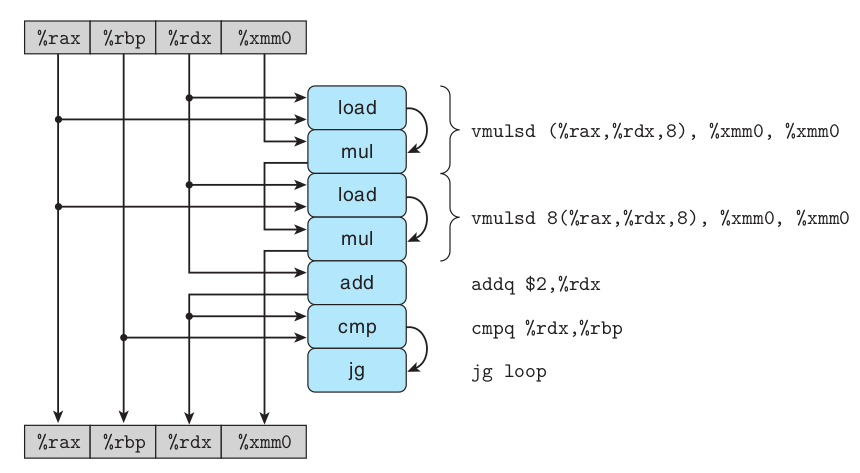
\includegraphics[width=\textwidth]{img/5-5}
        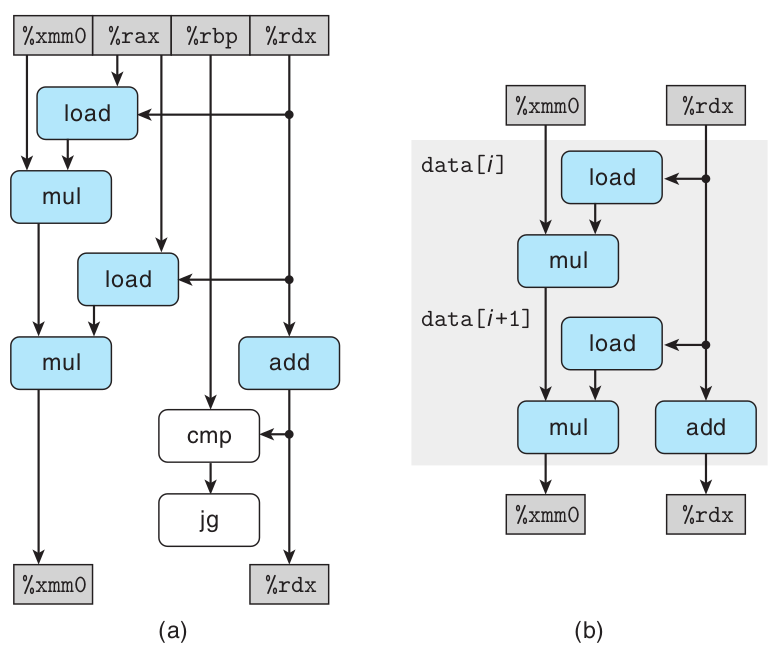
\includegraphics[width=0.9\textwidth]{img/5-6}
    \end{minipage}
    \begin{minipage}{0.33\textwidth}
        \centering
        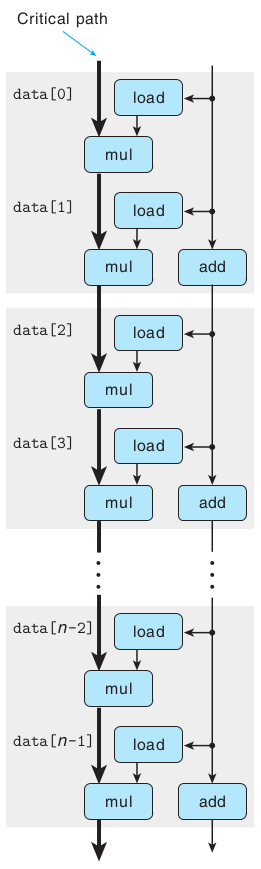
\includegraphics[width=\textwidth]{img/5-7}
    \end{minipage}
\end{figure}

可以看到,关键路径还是 n 个 mul 操作,虽然迭代次数减半了,但是每次迭代中有两个顺序的乘法操作。这个关键路径是循环没有展开代码的性能制约因素,而它仍然是 $k \times 1$ 循环展开代码的性能制约因素。

\section{提高并行性}

在此,程序的性能是受运算单元的延迟限制的。由于执行加法和乘法的功能单元是完全流水化的,这意味着它们可以每个时钟周期开始一个新操作,并且有些操作可以被多个功能单元执行。硬件具有以更高速率执行乘法和加法的潜力,但是代码不能利用这种能力,既是是使用循环展开也不能,这是因为我们将累计值放在一个单独的变量 acc 中。在前面的计算完成之前,都不能计算 acc 的新值。

\subsection{多个累计变量}

对于一个可结合和可交换的 combine 运算来说,我们可以通过将一组 combine 运算分割成两个或更多的部分,并在最后合并结果来提高性能。例如,$P_n$ 表示元素 $a_0, a_1, \cdots, a_{n-1}$ 的乘积:

\[
    P_n = \prod_{i=0}^{n-1} a_i
\]

假设 n 为偶数,还可以把它写成 $P_n = PE_n \times PO_n$,这里 $PE_n$ 是索引值为偶数的元素的乘积,而 $PO_n$ 是索引值为奇数的元素的乘积:

\begin{align*}
    PE_n & = \prod_{i=0}^{n/2-1} a_{2i} \\
    PO_n & = \prod_{i=0}^{n/2-1} a_{2i+1}
\end{align*}

下面是使用这种方法的代码。它既使用了两次循环,以使每次迭代合并更多的元素,也使用了两路并行,将索引值为偶数的元素累积在变量 acc0 中,而索引值为奇数的元素累积在变量 acc1 中。因此,我们将其称为 $2 \times 2$ 循环展开。

\begin{minted}{cpp}
// 2 x 2 loop unrolling
void combine6(vec_ptr v, data_t *dest) {
  long i;
  long length = vec_length(v);
  long limit = length - 1;
  data_t *data = get_vec_start(v);
  data_t acc0 = IDENT;
  data_t acc1 = IDENT;

  // Combine 2 elements at a time
  for (i = 0; i < limit; i += 2) {
    acc0 = acc0 OP data[i];
    acc1 = acc1 OP data[i+1];
  }

  // Finish any remaining elements
  for (; i < length; ++i) {
    acc0 = acc0 OP data[i];
  }
  *dest = acc0 OP acc1;
}
\end{minted}

可以得到下面的性能:

\begin{table}[!ht]
    \centering
    \begin{tabular}{llccccc}
        \toprule
        & & \multicolumn{2}{c}{Integer} & & \multicolumn{2}{c}{Floating point} \\
        \cmidrule{3-4} \cmidrule{6-7}
        Function & Method & + & * & & + & * \\
        \midrule
        \texttt{combine4} & Accumulate in temporary & 1.27 & 3.01 & & 3.01 & 5.01 \\
        \texttt{combine5} & $2 \times 1$ unrolling & 1.01 & 3.01 & & 3.01 & 5.01 \\
        \texttt{combine6} & $2 \times 2$ unrolling & 0.81 & 1.51 & & 1.51 & 2.51 \\
        \\
        Latency bound & & 1.00 & 3.00 & & 3.00 & 5.00 \\
        Throughput bound & & 0.50 & 1.00 & & 1.00 & 0.50 \\
        \bottomrule
    \end{tabular}
\end{table}

要理解 combine6 的性能,我们从下图所示的代码和操作序列开始。同 combine5 一样,这个内循环包括两个 vmulsd 运算,但是这些指令被翻译成读写不同寄存器的 mul 操作,它们之间没有数据相关。然后,把这个模板复制 n/2 次,就是在一个长度为 n 的向量上执行这个函数的模型。可以看到,现在有两条关键路径,一条对应于计算索引为偶数的元素的乘积(acc0),另一条对应于计算索引为奇数的元素的乘积(acc1),每条关键路径只包含 n/2 个操作。

\begin{figure}[!ht]
    \centering
    \begin{minipage}{0.65\textwidth}
        \centering
        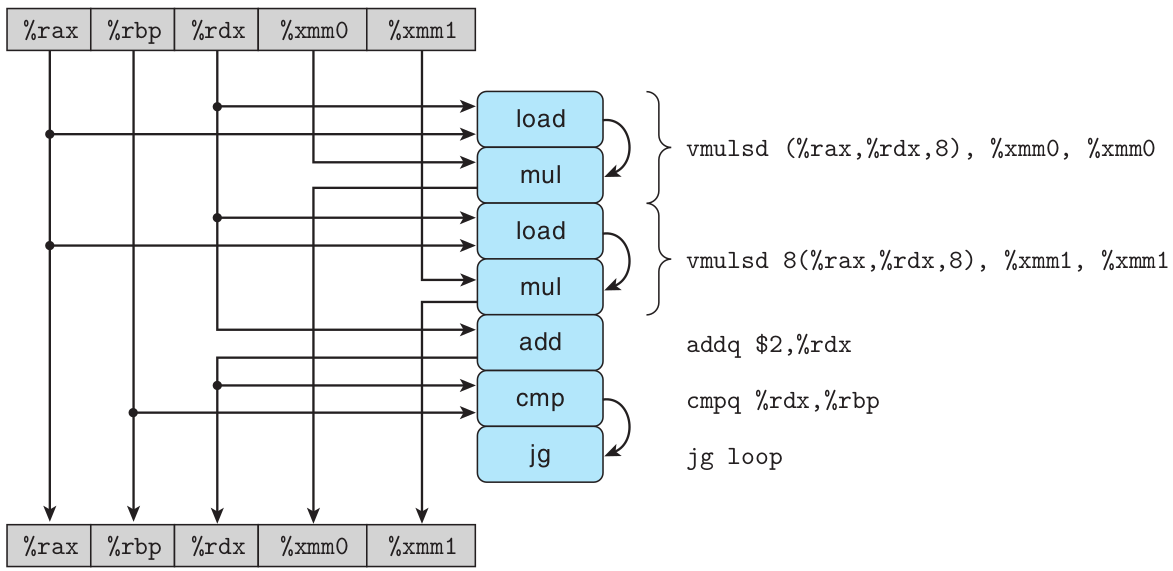
\includegraphics[width=\textwidth]{img/5-8}
        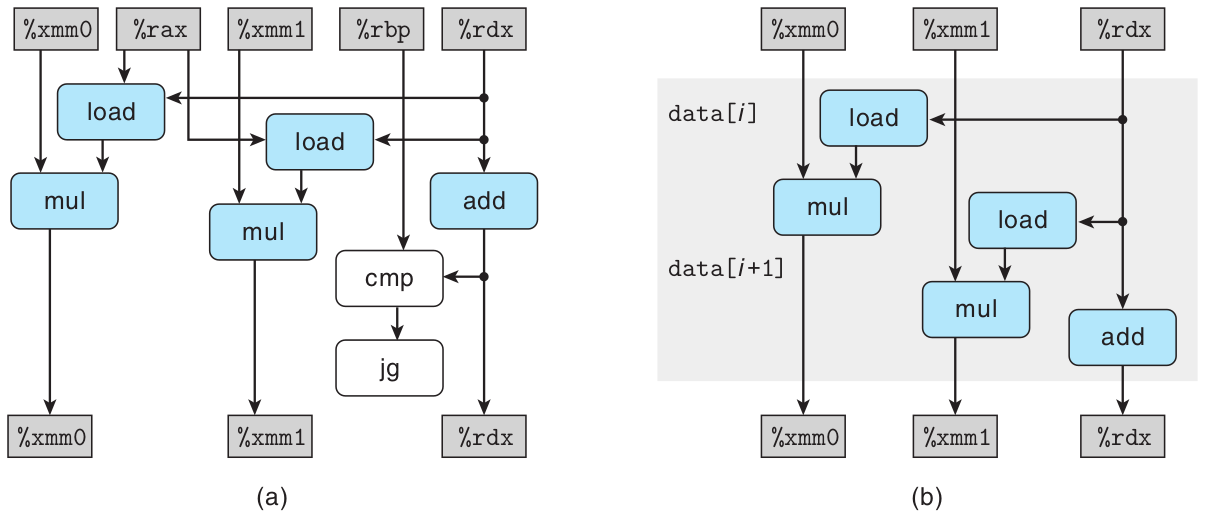
\includegraphics[width=\textwidth]{img/5-9}
    \end{minipage}
    \begin{minipage}{0.33\textwidth}
        \centering
        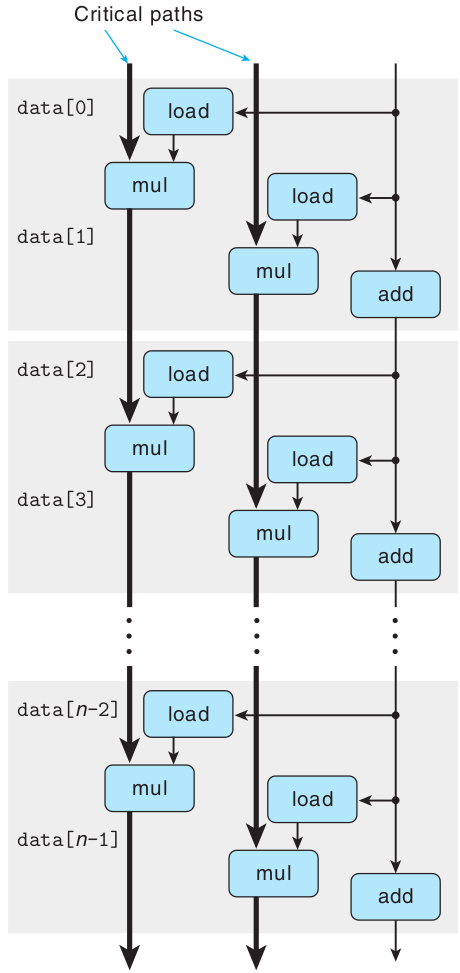
\includegraphics[width=\textwidth]{img/5-10}
    \end{minipage}
\end{figure}

我们可以将多个累积变量变换归纳为将循环展开 $k$ 次,以及并行累积 $k$ 个值,得到 $k \times k$ 循环展开。通常,只有保持能够执行该操作的所有功能单元的流水线都是满的,程序才能达到这个操作的吞吐量界限。对延迟为 $L$,容量为 $C$ 的操作而言,这就要求循环展开因子 $k \geq C \cdot L$。

在执行 $k \times k$ 循环展开变换时,必须考虑是否要保留原始函数的功能。补码运算是可交换和可结合的,因此,对于整数数据类型,在所有可能的情况下,combine6 计算出的结果都和 combine5 计算出的结果相同。因此,优化编译器潜在地能够将 combine4 中所示的代码首先转换成 combine5 的二路循环展开的版本,然后再通过引入并行性,将之转换成 combine6 的版本。另一方面,浮点乘法和加法不是可结合的,大多数编译器不会尝试对浮点代码进行转换。

\subsection{重新结合变换}

现在来探讨另一种打破顺序相关从而使性能超过延迟界限的方法。我们看到过做 $k \times 1$ 循环展开的 combine5 的数据相关,对代码做很小的改动,可以从根本改变合并执行的方式,也极大地提高了程序的性能。

下面给出了 combine7,它与 combine5 的展开代码的唯一区别在于内循环中元素合并的方式。在 combine5 中,合并是以下面这条语句来实现的:
\begin{minted}[linenos=false]{cpp}
    acc = (acc OP data[i]) OP data[i+1];
\end{minted}
而在 combine7 中,合并是以这条语句来实现的:
\begin{minted}[linenos=false]{cpp}
    acc = acc OP (data[i] OP data[i+1]);
\end{minted}
差别仅在于两个括号是如何放置的。我们称之为 reassociation transformation(重新结合变换),因为括号改变了向量元素与累积值 acc 的合并顺序,产生了我们称为 $2 \times 1a$ 的循环展开形式。

\begin{minted}{cpp}
// 2 x 1a loop unrolling
void combine7(vec_ptr v, data_t *dest) {
  long i;
  long length = vec_length(v);
  long limit = length - 1;
  data_t *data = get_vec_start(v);
  data_t acc = IDENT;

  // Combine 2 elements at a time
  for (i = 0; i < limit; i += 2) {
    acc = acc OP (data[i] OP data[i+1]);
  }

  // Finish any remaining elements
  for (; i < length; ++i) {
    acc = acc OP data[i];
  }
  *dest = acc;
}
\end{minted}

\begin{figure}[!ht]
    \centering
    \begin{minipage}{0.65\textwidth}
        \centering
        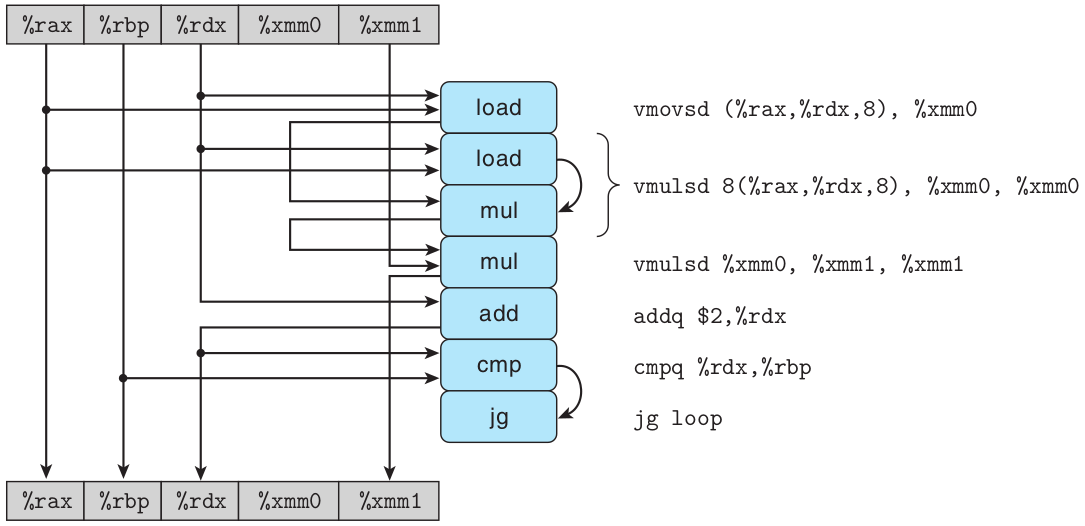
\includegraphics[width=\textwidth]{img/5-11}
        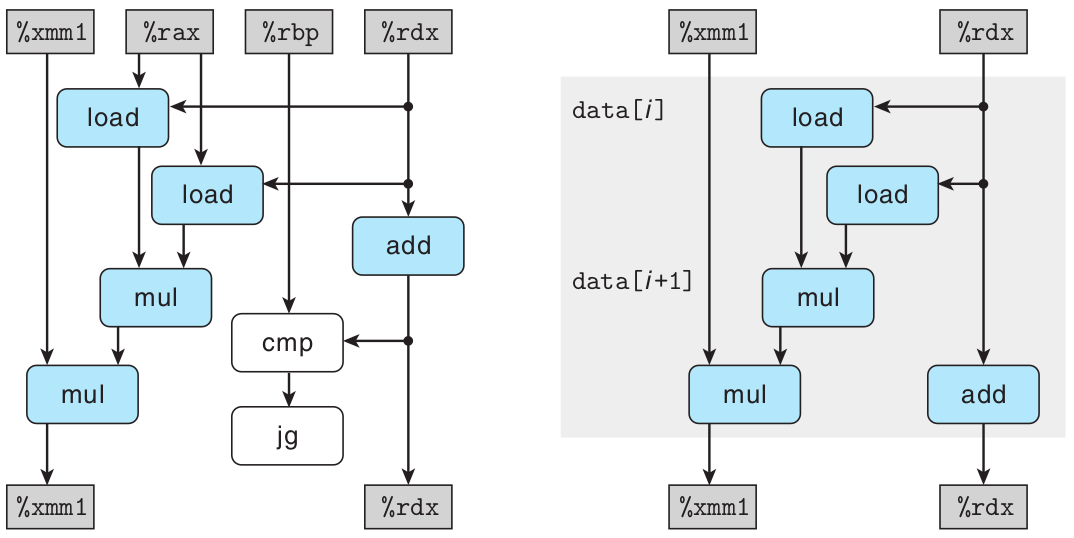
\includegraphics[width=\textwidth]{img/5-12}
    \end{minipage}
    \begin{minipage}{0.33\textwidth}
        \centering
        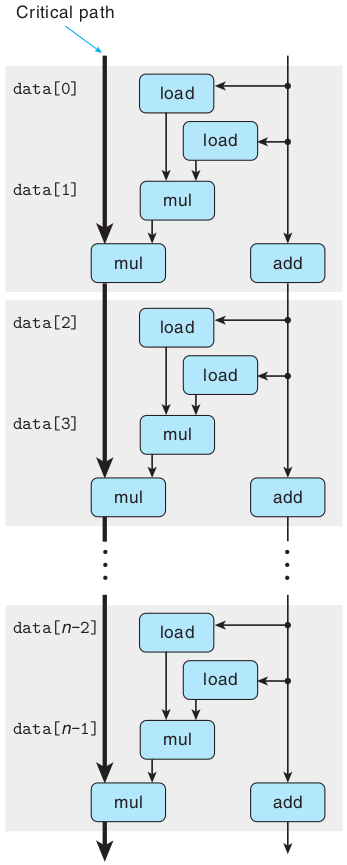
\includegraphics[width=\textwidth]{img/5-13}
    \end{minipage}
\end{figure}

\begin{table}[!ht]
    \centering
    \begin{tabular}{llccccc}
        \toprule
        & & \multicolumn{2}{c}{Integer} & & \multicolumn{2}{c}{Floating point} \\
        \cmidrule{3-4} \cmidrule{6-7}
        Function & Method & + & * & & + & * \\
        \midrule
        \texttt{combine4} & Accumulate in temporary & 1.27 & 3.01 & & 3.01 & 5.01 \\
        \texttt{combine5} & $2 \times 1$ unrolling & 1.01 & 3.01 & & 3.01 & 5.01 \\
        \texttt{combine6} & $2 \times 2$ unrolling & 0.81 & 1.51 & & 1.51 & 2.51 \\
        \texttt{combine7} & $2 \times 1a$ unrolling & 1.01 & 1.51 & & 1.51 & 2.51 \\
        \\
        Latency bound & & 1.00 & 3.00 & & 3.00 & 5.00 \\
        Throughput bound & & 0.50 & 1.00 & & 1.00 & 0.50 \\
        \bottomrule
    \end{tabular}
\end{table}

除了整数加外,都突破了延迟界限造成的限制。上图说明了 combine7 内循环的代码是如何被译码成操作,以及由此得到的数据相关。可以看到关键路径上只有 n/2 个操作,每次迭代内的第一个乘法都不需要等待前一次迭代的累积值就可以执行,因此,最小可能的 CPE 就减少了 2 倍。

重新结合变换能够减少计算中关键路径上操作的数量,通过更好地利用功能单元的流水线能力得到更好的性能。大多数编译器不会尝试对浮点运算做重新结合被,因为这些运算不保证是可结合的。

\section{优化合并代码的结果小结}

下表总结了对于标量代码所获得的结果,没有使用 AVX 向量指令提供的向量并行性:

\begin{table}[!ht]
    \centering
    \begin{tabular}{llccccc}
        \toprule
        & & \multicolumn{2}{c}{Integer} & & \multicolumn{2}{c}{Floating point} \\
        \cmidrule{3-4} \cmidrule{6-7}
        Function & Method & + & * & & + & * \\
        \midrule
        \texttt{combine1} & Abstract -O1 & 10.12 & 10.12 & & 10.17 & 11.14 \\
        \texttt{combine6} & $2 \times 2$ unrolling & 0.81 & 1.51 & & 1.51 & 2.51 \\
                        & $10 \times 10$ unrolling & 0.55 & 1.00 & & 1.01 & 0.52 \\
        \\
        Latency bound & & 1.00 & 3.00 & & 3.00 & 5.00 \\
        Throughput bound & & 0.50 & 1.00 & & 1.00 & 0.50 \\
        \bottomrule
    \end{tabular}
\end{table}

使用多项优化技术,我们获得的 CPE 已经接近于 0.50 和 1.00 的吞吐量界限,只受限于功能单元的容量。与原始代码相比提升了 10 \~{} 20 倍,且使用普通的 C 代码和标准编译器就获得了所有这些改进。这个例子说明现代处理器具有相当的计算能力,但是我们可能需要按非常程式化的方式来编写程序以便将这些能力诱发出来。

\section{一些限制因素}

我们已经看到在一个程序的数据流图表示中,关键路径已经指明了执行该程序所需时间的一个基本的下界。也就是说,如果程序中有某条数据相关链,这条链上的所有延迟之和等于 $T$,那么这个程序至少需要 $T$ 个 周期才能执行完。

我们还看到功能单元的吞吐量界限也是程序执行时间的一个下界。也就是说,假设一个程序需要 $N$ 个某种运算的计算,而微处理器只有 $C$ 个能执行这个操作的功能单元,并且这些单元的发射时间为 $I$。那么,这个程序的执行至少需要 $N \cdot I / C$ 个周期。

在本节中,我们会考虑其他一些制约程序在实际机器上性能的因素。

\subsection{寄存器溢出}

循环并行性的好处受汇编代码描述计算的能力限制。如果我们的并行度 p 超过了可用的寄存器数量,那么编译器会诉诸溢出(spilling),将某些临时值存放到内存中,通常是在运行时堆栈上分配空间。

\begin{table}[!ht]
    \centering
    \begin{tabular}{llccccc}
        \toprule
        & & \multicolumn{2}{c}{Integer} & & \multicolumn{2}{c}{Floating point} \\
        \cmidrule{3-4} \cmidrule{6-7}
        Function & Method & + & * & & + & * \\
        \midrule
        \texttt{combine6} & $10 \times 10$ unrolling & 0.55 & 1.00 & & 1.01 & 0.52 \\
                          & $20 \times 20$ unrolling & 0.83 & 1.03 & & 1.02 & 0.68 \\
        \\
        Latency bound & & 1.00 & 3.00 & & 3.00 & 5.00 \\
        Throughput bound & & 0.50 & 1.00 & & 1.00 & 0.50 \\
        \bottomrule
    \end{tabular}
\end{table}

可以看到对这种循环展开程度的增加没有改善 CPE,甚至还变差了。
